\documentclass[12pt]{ucthesis}

%\newif\ifpdf
%\ifx\pdfoutput\undefined
%    \pdffalse % we are not running PDFLaTeX
%\else
%\pdfoutput=1 % we are running PDFLaTeX
%\pdftrue \fi

\usepackage{url}

%\ifpdf

    \usepackage[pdftex]{graphicx}
    % Update title and author below...
    \usepackage[pdftex,plainpages=false,breaklinks=true,colorlinks=true,urlcolor=blue,citecolor=blue,%
                                       linkcolor=blue,bookmarks=true,bookmarksopen=true,%
                                       bookmarksopenlevel=3,pdfstartview=FitV,
                                       pdfauthor={John Smith},
                                       pdftitle={PDF Title},
                                       pdfkeywords={thesis, masters, cal poly}
                                       ]{hyperref}
    %Options with pdfstartview are FitV, FitB and FitH
    \pdfcompresslevel=1

%\else
%    \usepackage{graphicx}
%\fi

\usepackage{amssymb}
\usepackage{amsmath}
\usepackage{mathtools}
\usepackage[letterpaper]{geometry}
\usepackage[overload]{textcase}
\usepackage{graphicx}
\usepackage{url}
\usepackage{titlesec}
\usepackage{etoolbox}
\usepackage[section]{placeins}
\usepackage{background}
\usepackage{lipsum}
\usetikzlibrary{calc}
\SetBgScale{1}
\SetBgAngle{0}
\SetBgColor{black}
\SetBgContents{

\begin{tikzpicture}[overlay,remember picture]
    \draw [line width=1pt,rounded corners=10pt,double]
        ($ (current page.north west) + (1cm,-1cm) $)
        rectangle
        ($ (current page.south east) + (-1cm,1cm) $);
\end{tikzpicture}
}




%\bibliographystyle{abbrv}

\setlength{\parindent}{0.25in} \setlength{\parskip}{3pt}

\geometry{verbose,nohead,tmargin=1.25in,bmargin=1in,lmargin=1in,rmargin=1in}

\setcounter{tocdepth}{2}


% Different font in captions (single-spaced, bold) ------------
\newcommand{\captionfonts}{\small\bf\ssp}

\makeatletter  % Allow the use of @ in command names
\long\def\@makecaption#1#2{%
  \vskip\abovecaptionskip
  \sbox\@tempboxa{{\captionfonts #1: #2}}%
  \ifdim \wd\@tempboxa >\hsize
    {\captionfonts #1: #2\par}
  \else
    \hbox to\hsize{\hfil\box\@tempboxa\hfil}%
  \fi
  \vskip\belowcaptionskip}
\makeatother   % Cancel the effect of \makeatletter
% ---------------------------------------




\begin{document}

% Declarations for Front Matter

% Update fields below!
\title{Cal Poly Thesis}
\author{John Smith}
\degreemonth{June} \degreeyear{2015} \degree{Master of Science}
\defensemonth{June} \defenseyear{2015}
\numberofmembers{4} 
\chair{Ernest Merkel, Ph.D. \\ & Associate Professor \\ & Statistics Department} 
\othermemberA{Kathy Abernathy, Ph.D.\\ & Associate Professor \\ & Engineering Department} 
\othermemberB{Peter Chan, Ph.D.\\ &  Associate Professor \\ & Mathematics Department}
\othermemberC{Jason Pearson, Ph.D.\\ & Professor \\ & Chemistry Department} 
\field{Electrical Engineering} 
\campus{San Luis Obispo}
\copyrightyears{seven}



\maketitle
\iftrue
\begin{frontmatter}

%\copyrightpage

%\committeemembershippage

\iffalse
\begin{abstract}
Your abstract goes here. 
%Leave the vspace below alone.
\vspace*{-12pt}
\end{abstract}

\begin{acknowledgements}

Add any acknowledgements here.

\end{acknowledgements} 
\fi


\tableofcontents


%\listoftables

\listoffigures

\end{frontmatter}
\fi
\pagestyle{plain}


\renewcommand{\baselinestretch}{1}

\titleformat{\chapter}[display]
    {\normalfont\huge\bfseries}{\chaptertitlename\ \thechapter}{20pt}{\Huge}
\titlespacing*{\chapter}{0pt}{-5pt}{10pt}

\makeatletter
\patchcmd{\chapter}{\if@openright\cleardoublepage\else\clearpage\fi}{}{}{}
\makeatother


% ------------- Main chapters here --------------------
\chapter{Introduction}
\label{intro}
Since the creation of Internet, World Wide Web (WWW) is one of the most widely used information sharing network. However, over the last few years,``Social Media Websites'' have the become most well-known and widely used tools for information sharing. Some of the widely used social networking sites are, Facebook (1.28 billion monthly active users), Twitter (271 million monthly active users) and LinkedIn (277 million members).
  
 In the social networking websites, the user joins a network and make ``connections'' by creating links with the other users in the network and interacts with them. Social media is an extensive source for interaction from everyday observations to elaborate discussions. The widespread popularity and rapid growth of these online social networks encourages us to study its properties and impact. Study of currently available online social networks is useful to design future online social network based systems considering its effect on the Internet. Also, by superlative analysis of social networks, we get the knowledge about information propagation, new directions for information search and concentration of information.

  
 The primary goal of the project henceforth is to understand the use of available social network analysis tools. After extensive search for social network analysis tools, we found the best tool for analyzing Facebook data to be ``Personal Analytics for Facebook - Wolfram Alpha'' and the best tool for analyzing Twitter data to be ``Twitalyzer''. In this project, we present these tools and understand the structure of social network data by doing the constructive analysis of the represented graphs. In addition to these, we find the pros and cons of these tools with respect to the different domain of users and application requirements.
 
 We also develop a prototype for a tool ``Personal Social Media Analysis Tool'' alias ``PERSMA'', which addresses the shortcomings of the available online analysis tools and provide more  innovative analysis of social networks. This tool will be later enhanced in Project 2, whereby we will provide the user with new representations and features like  connectivity of followers/friends, predictive analysis, free usage of the tool etc.
 
 In the next chapters, we will describe the analysis of ``Personal Analytics for Facebook - Wolfram Alpha'' and ``Twitalyzer'' tools, as well as Architectural flow and implementation details of PERSMA.

\chapter{Online Social Media Analysis Tools}
\section{Facebook}
Wolfram Alpha \cite{wolfram} is not only a search engine, but also a “computational knowledge engine” that helps people find what they need. Wolfram Alpha uses its expert-level knowledge to answer questions generating results that contains various reports and analysis across domains. The newest domain being ``Social Network'' for which Wolfram Alpha has developed a comprehensive tool i.e. ``Personal Analytics for Facebook - Wolfram Alpha''. The highlight of the tool is its ease of use and most of the features of this tool are free. The user only needs to sign in by providing the Facebook credentials and the tool generates the report.

Here are some of the details about the features and graphs of ``Personal Analytics for Facebook - Wolfram Alpha'' tool:
  
\begin{itemize}
\item \textbf{Word Cloud:}
	Word Cloud gives the basic idea about what the user talks more on Facebook as seen in the figure \ref{WordCloud}. It gives the essence about the most common words the user uses in Facebook wall posts. Bigger the size of the word, the more often it is used in conversations. Also, user's interests can be deduced from the word cloud analysis.
 \begin{figure}[!htb]
   	\centering
    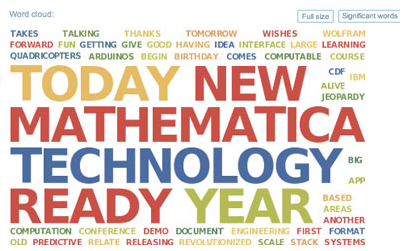
\includegraphics[height=55mm]{WolframWordCloud.PNG}
    \captionfonts
    \caption[Word Cloud]{Word Cloud}
    \label{WordCloud}
  \end{figure}

\item \textbf{Color Coded Friend Network:}
	Wolfram Alpha presents the user's Facebook data in color coded clusters represented by little circles and different color codes as shown in the figure \ref{ColorCodedFriendNetwork}. As the mouse hovers on these little circles, the user gets brief details about friend's identity. And after clicking on these circles; it takes the user to respective Facebook profile. The color coded friend network classifies friends into five different ``network roles'' which are social insiders, social outsiders, social neighbors, social gateways, and social connectors. Social insiders are people who have a lot of friends in common with the user. Whereas, Social outsiders is opposite of social insiders i.e. social outsider is a person with whom the user have very few or almost no mutual friends.
 
	Social gateways are the people who have a lot of friends that are outside of user's network. Social neighbors are opposite of Social gateways i.e. social neighbor is a person who has very few friends outside of user's network. Social connectors are the people in user's network who connect two separate groups of friends i.e. those who connect friends from the school and college. Along with these properties, the color coded network can be categorized using interesting features such as age, relationship status, gender, number of likes, number of comments etc. From this analysis, the user can know the best social connector to connect different group of friends.
\begin{figure}[!htb]
\centering
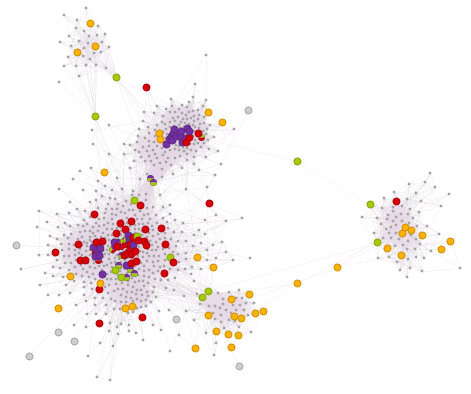
\includegraphics[height=90mm]{WolframColorCodedNetwork.PNG}
\captionfonts
\caption[Color Coded Friend Network]{Color Coded Friend Network}
\label{ColorCodedFriendNetwork}
\end{figure}

\item \textbf{Most Popular Photo:}
	As shown in the figure \ref{MostPopularPhoto} Wolfram Alpha gives the brief analysis of both the most liked and most commented photo from the user's Facebook data because it is not necessary that the most commented photo is same as the most liked photo. Here, it shows the most commented photo along with its attributes such as caption of the photo, the date on which it was added, the album in which it's added, and number of comments on the photo. It also includes the details about people tagged in the photo. Similarly, these attributes are shown separately for the most liked photo.
\begin{figure}[!htb]
\centering
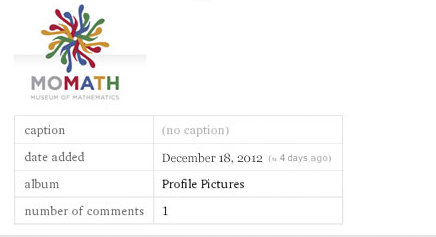
\includegraphics{WolframMostCommentedPhoto.PNG}
\captionfonts
\caption[Most Popular Photo]{Most Popular Photo}
\label{MostPopularPhoto}
\end{figure} 
\item \textbf{Friend Network:}	
	This is one of the more intriguing graph Wolfram Alpha generates for user's friend network as shown in the figure \ref{FriendNetwork}. It classifies friend network into various clusters depending on the variety of categories such as friends from schools, colleges, colleagues, family or relatives and so on. The size of the cluster shows the number of friends in it. Bigger the size of the cluster, more number of friends are from specific group. The graph also shows the relationship between various clusters. The distance between the clusters gives the intuition about how closely people in the clusters are connected to each other.
\begin{figure}[!htb]
\centering
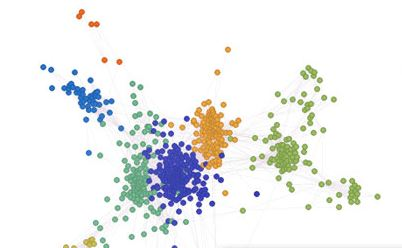
\includegraphics[height=65mm,width=150mm]{WolframFriendNetwork.JPG}
\captionfonts
\caption[Friend Network]{Friend Network}
\label{FriendNetwork}
\end{figure}
\end{itemize}
\section{Twitter}
In this section we review the analysis provided by one of the comprehensive tools available online for Twitter Data Analysis called Twitalyzer \cite{twitalyzer}. This tool is focused on generating reports for Enterprise clients who use these analysis for targetting audience for their product and services. As a result of which it is a paid service and hence the following tool features and images are referenced from the sample reports available online \cite{twitalyzer_ex}.  

\begin{itemize}
  \item \textbf{Comparision Chart:} The tool provides you a complete comparision of you and your peers on various social parameters like Influence, Engagement etc. as seen in the figure \ref{twitcomp}. 
  This helps one to compare yourself and gain insight on one's strong and weak points and hence the users can set goals for themselves to achieve in terms of these social parameters. 
  
  \begin{figure}[!htb]
  \begin{center}
  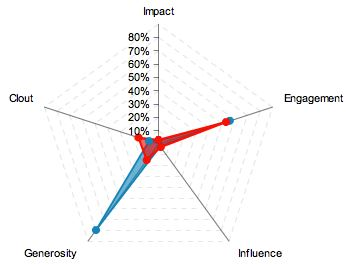
\includegraphics[height=60mm, width=80mm]{twit_compare.JPG}
  \captionfonts
  \caption[Twitter Comparision]{Twitter Comparision on Social Parameters}
  \label{twitcomp}
  \end{center}
  \end{figure}%

  \item \textbf{Network Explorer:} This representation provides insight into how one is connected to different people and topics (hashtags) on the twitter. This figure \ref{netexplorer} shows the strength of connection by the weight(thickness) of the line connecting two entities. This helps in monitoring what topics one generally engages in and what people they are strongly connected to. 
  Additional insight that can be gained from this type of graph is the degree of separation between you and other people and topics.  
  
  \begin{figure}[!htb]
  \begin{center}
  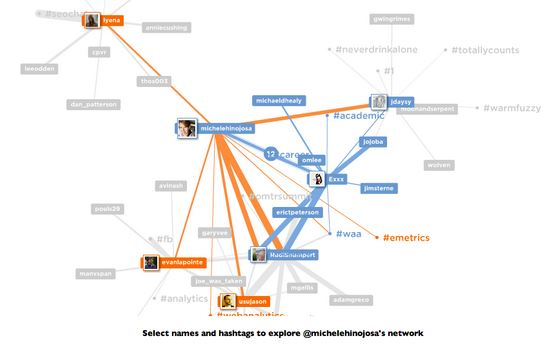
\includegraphics[height=70mm, width=.99\linewidth]{netework.JPG}
  \captionfonts
  \caption[Network Explorer]{Network Explorer}
  \label{netexplorer}
  \end{center}
  \end{figure}%
  
  \item \textbf{Network Activity:} This cool chart gives you the analysis about when most of your network is online. As can be seen in figure \ref{netactivity}, the number of active users are represented by different colors for a period of one week throughout the day. 
  This gives one insight into when some activity like a tweet for promotion would get maximum response from the network. 
  
  \begin{figure}[!htb]
  \begin{center}
  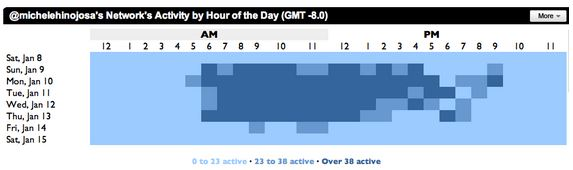
\includegraphics[height=40mm, width=.99\linewidth]{network_activity.JPG}
  \captionfonts
  \caption[Network Activity]{Network Activity}
  \label{netactivity}
  \end{center}
  \end{figure}%
  
  \item \textbf{Sentiment Analysis:} This analysis is similar to the word cloud analysis for Facebook by Wolfram. In which it categorizes the words used by the user into positive and negative sentiments and analyzes them on a time period to track which sentiments are mainly used and how they change over the time.
  The figure \ref{sentanalysis} shows how positive sentiments are higher on Friday than compared to the following Sunday. This analysis gives you not only analysis about the tweets and their timings and influence but also analysis about the content of the tweets.\\
  
  \begin{figure}[!htb]
  \begin{center}
  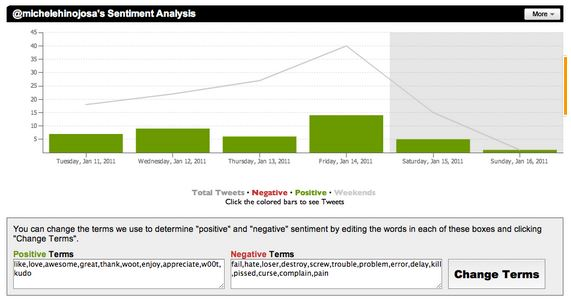
\includegraphics[height=70mm, width=.99\linewidth]{sentimentanalysis.JPG}
  \captionfonts
  \caption[Sentiment Analysis]{Sentiment Analysis}
  \label{sentanalysis}
  \end{center}
  \end{figure}%
  
\end{itemize}

\chapter{PERSMA}
\label{ch2}

\section{Motivation}
\label{ch2s1}
Based on the initial survey of the existing tools we have found the following features that are missing from them. 
\begin{itemize}
\item As seen so far, the analysis of Social Media is focused on business clients and most of the services are paid. For students and people interested in analyzing their data on a small scale these services are not feasible. 
\item There is no comprehensive analysis tool which uses data from multiple social networks to give more insight into one's social network personality. 
\item The analysis is done in a statistical manner and graphs are generated based on the data observed over a period of time. There are no sophisticated predictions made on the observed data to provide better service. 
\end{itemize}

This gave us the motivation to build a new tool for Personal Social Media Analysis that would be used by general public and students like us interested in social network analysis for free of cost. This tool in the scope of this semester would provide integration of data from two popular social networking sites Facebook and Twitter. It would also provide simple prediction analysis of the observed data. 


\section{Architecture}
\label{ch2s2}
\begin{figure}[ht!]
\begin{center}
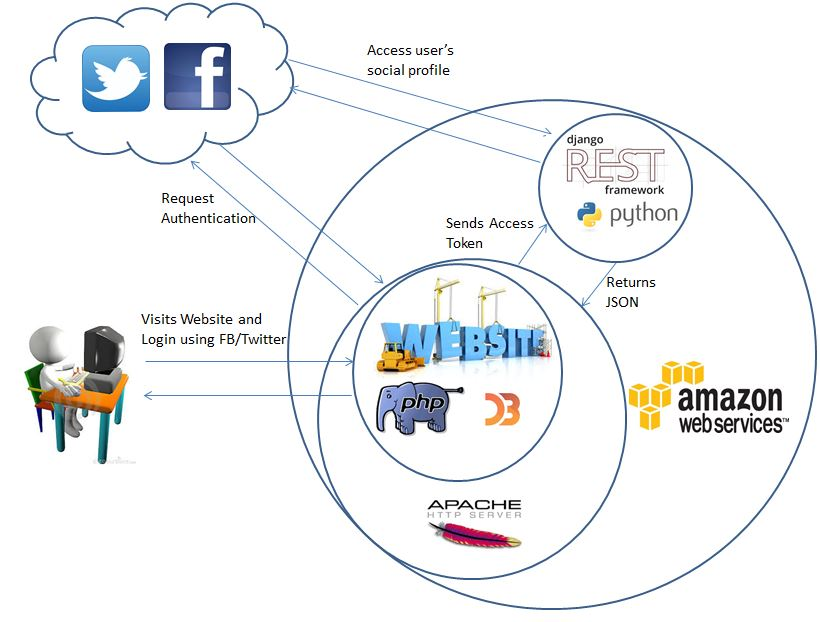
\includegraphics[height=100mm]{arch.JPG}
\captionfonts
\caption[Architecture Diagram of PERSMA]{Architecture Diagram for PERSMA}
\label{arch}
\end{center}
\end{figure}

Some of the components in the architecture diagram are explained as follows:

\begin{itemize}
  \item \textbf{Amazon Web Services(AWS)}: AWS provides one of the best cloud computing platforms. We use an EC2 instance in AWS as the host server for both the front end and the back end of the tool.
  \item \textbf{Apache Web Server}: Apache provides an implementation of HTTP(Web) server which is used to host the front end of the tool.
  \item \textbf{PHP}: PHP is a scripting and programming language widely used in the web development worldwide. We are using PHP to create the front end of the tool.
  \item \textbf{Data Driven Documents(D3)}: D3.js is a Javascript library used to provide creation and control of charts which are highly interactive and graphical. This is used as the charting library at the front end of the tool.
  \item \textbf{Django Rest Framework and Python}: Python is a really powerful programming and scripting language which has low latency for complex computations. Since, the plan of our project is to integrate modeling and prediction analysis in our tool, Python provides a lot of tools to accomplish the same. Hence our backend of the tool is written in Python. Since, the backend of the tool must make and receive REST calls, we needed to provide REST interface over Python. Django is one of the best frameworks written over Python to provide the REST functionality. Hence we have made use of it.
\end{itemize}

\section{Challenges}
Apart from the implementation challenges for the tool, there were lot of issues regarding accessing the Facebook and Twitter Api's via REST, which are relevant for data mining. These are described as follows:
\begin{itemize}
  \item \textbf{Restricted API's}: Even after providing access to the tool via twitter or Facebook api's, the tool might not get the user's friend's data because it might be possible that her friends have blocked their private data. This doesn't give the full analysis of user's social network.  
  \item \textbf{Rate Limits}: Twitter puts rate limit for most of its api's to restrict the access. These limits are really very low in the range of 15 queries/15 min. These low rate limits restricts the real time analysis of the network.
  \item \textbf{Privacy Issues}: Due to the growing concern regarding the privacy of its users, Facebook has blocked its apps to fetch the whole friend list of the authenticated user. The apps will only get the list of those friends who also have authorized the app themselves. This, as we can image, really restricts the analysis of the user's network.
\end{itemize}

\section{User Flow}
In accordance with the architecture of the tool, we created a prototype of it within the boundaries of the challenges as itemized above. In the current version of the tool, it provides the Twitter login for the user and then generates a mutual relationship chart among only the user's  first 14 followers since we are restricted by the api rate limit of 15 queries per 15 min. The flow of the tool is explained as follows:

Any user in the worldwide web visits the website \cite{persma} of the tool which is a publicly accessible url. The Website currently has login option for Twitter. Once the user clicks on the login button, she will be redirected to the Twitter's login page. Here, she enters her username and password. Once Twitter accepts her credentials, she can now authorize the app with the relevant permissions. She now will be redirected to our main page via Twitter and in turn our tool receives an access token and an access token key, which servers as user credentials for the tool to talk to Twitter later on.

Once the user is on the tool's main page, she will have an option to create different charts providing different features and analysis. Depending on the chart type selected, the website makes the appropriate REST call to the back end of the server which is a Django REST server with the access tokens. The server after receiving the request, calls the appropriate Twitter API's to get the required data and uses the access tokens for authentication. Once it gets the data back from Twitter, it processes the data and sends the relevant information back to the website in the form of JSON. This JSON is then rendered by D3.js libraries to create visually appealing charts.

Figure \ref{loginpage} shows the main web page of the tool in its current form which currently has  login button for the user's Twitter account. This webpage is a publicly accessible url which can be accessed by going to http://tinyurl.com/persma.\\
\begin{figure}[!htb]
\begin{center}
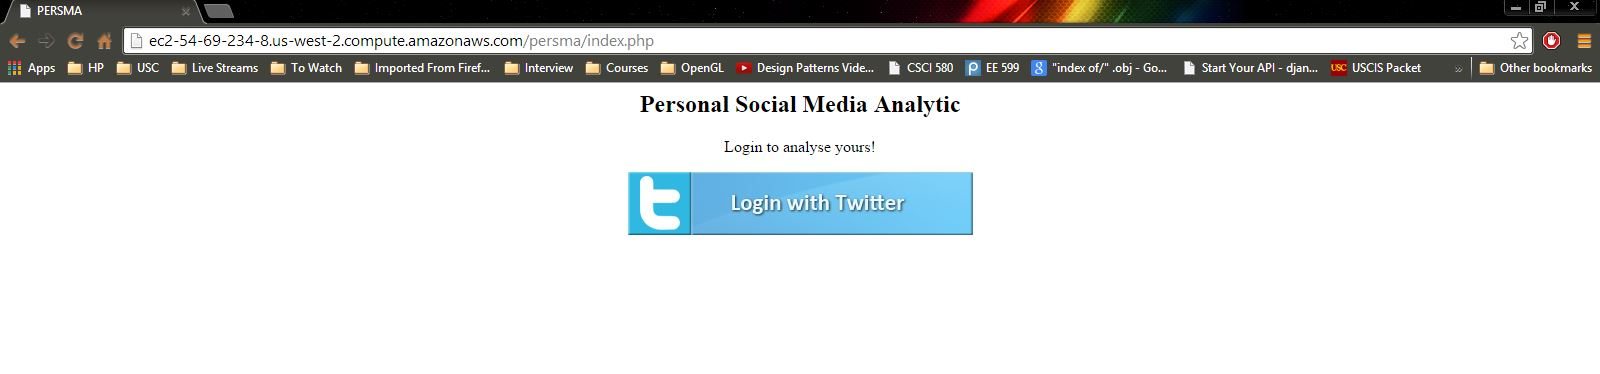
\includegraphics[height=70mm, width=.99\linewidth]{loginpage.JPG}
\captionfonts
\caption[Login Page]{Login Page}
\label{loginpage}
\end{center}
\end{figure}%
Once the user clicks on the login button for Twitter, she is redirected to the Twitter Web page as shown in figure \ref{authtwitterpage}. This page lets the user authorize the app by entering her Twitter credentials. On this page, the user can know what all permissions the app requires and what all user details the app is oblivious to.\\
\begin{figure}[!htb]
\begin{center}
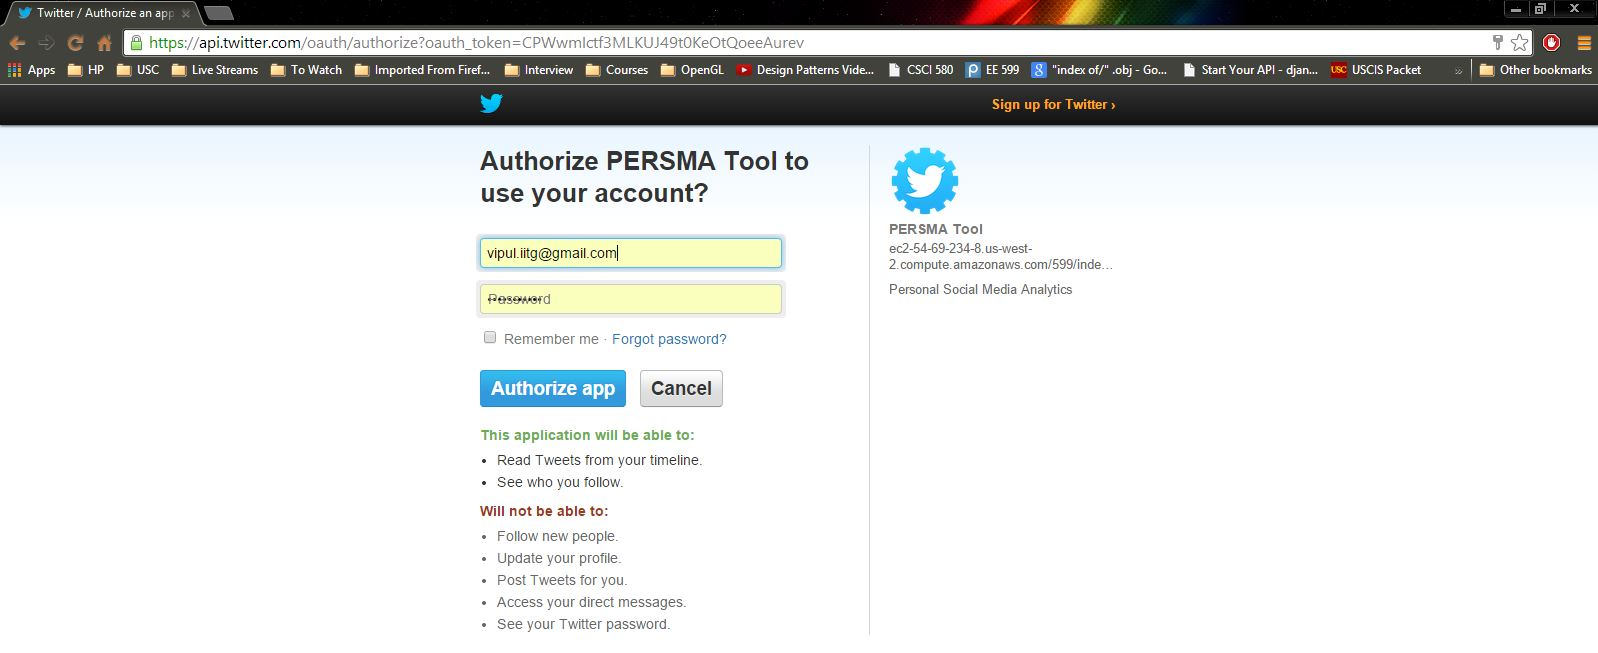
\includegraphics[height=50mm, width=.99\linewidth]{twitter_authorize.JPG}
\captionfonts
\caption[Authorization by Twitter]{Authorization by Twitter}
\label{authtwitterpage}
\end{center}
\end{figure}%
Once, the user has authenticated the app, she is redirected to the website's main page as shown in figure \ref{mainpage}. Once on main page, the user can see that her account details are now accessible to the tool. The website shows the user's name and profile picture which are loaded it on the main page. Now, the user can select the chart type to be displayed by clicking on the sidebar button on the left side of the screen, which expands the sidebar as depicted in figure \ref{selectgraph}.\\
\begin{figure}[!htb]
\centering
\begin{minipage}[b]{0.45\linewidth}
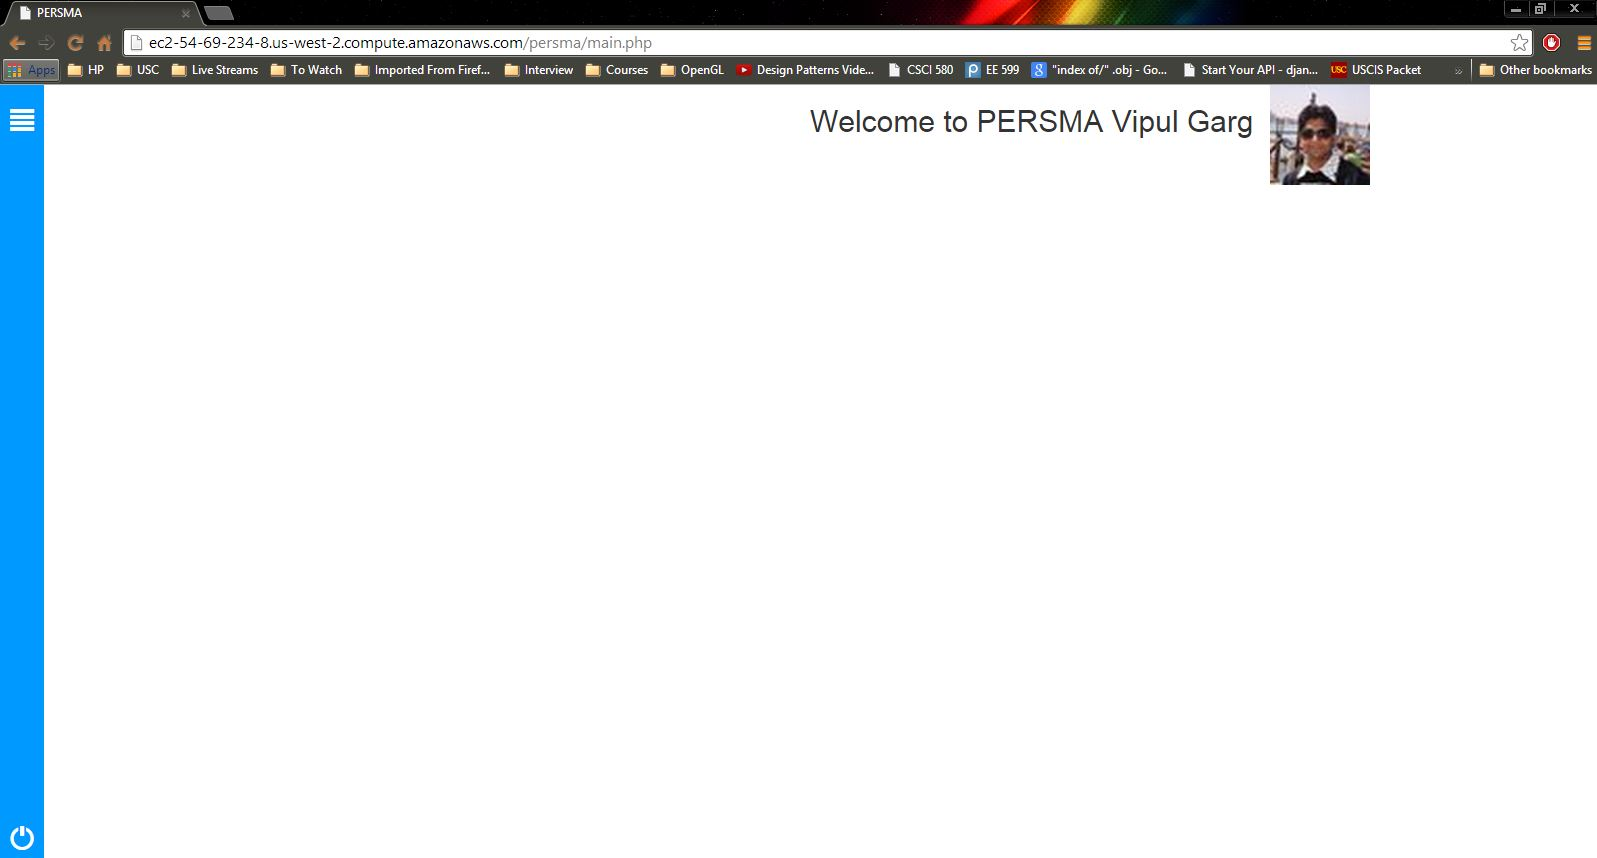
\includegraphics[height=40mm]{mainpage.JPG}
\captionfonts
\caption[Main Page]{Main Page}
\label{mainpage}
\end{minipage}%
\begin{minipage}[b]{0.45\linewidth}
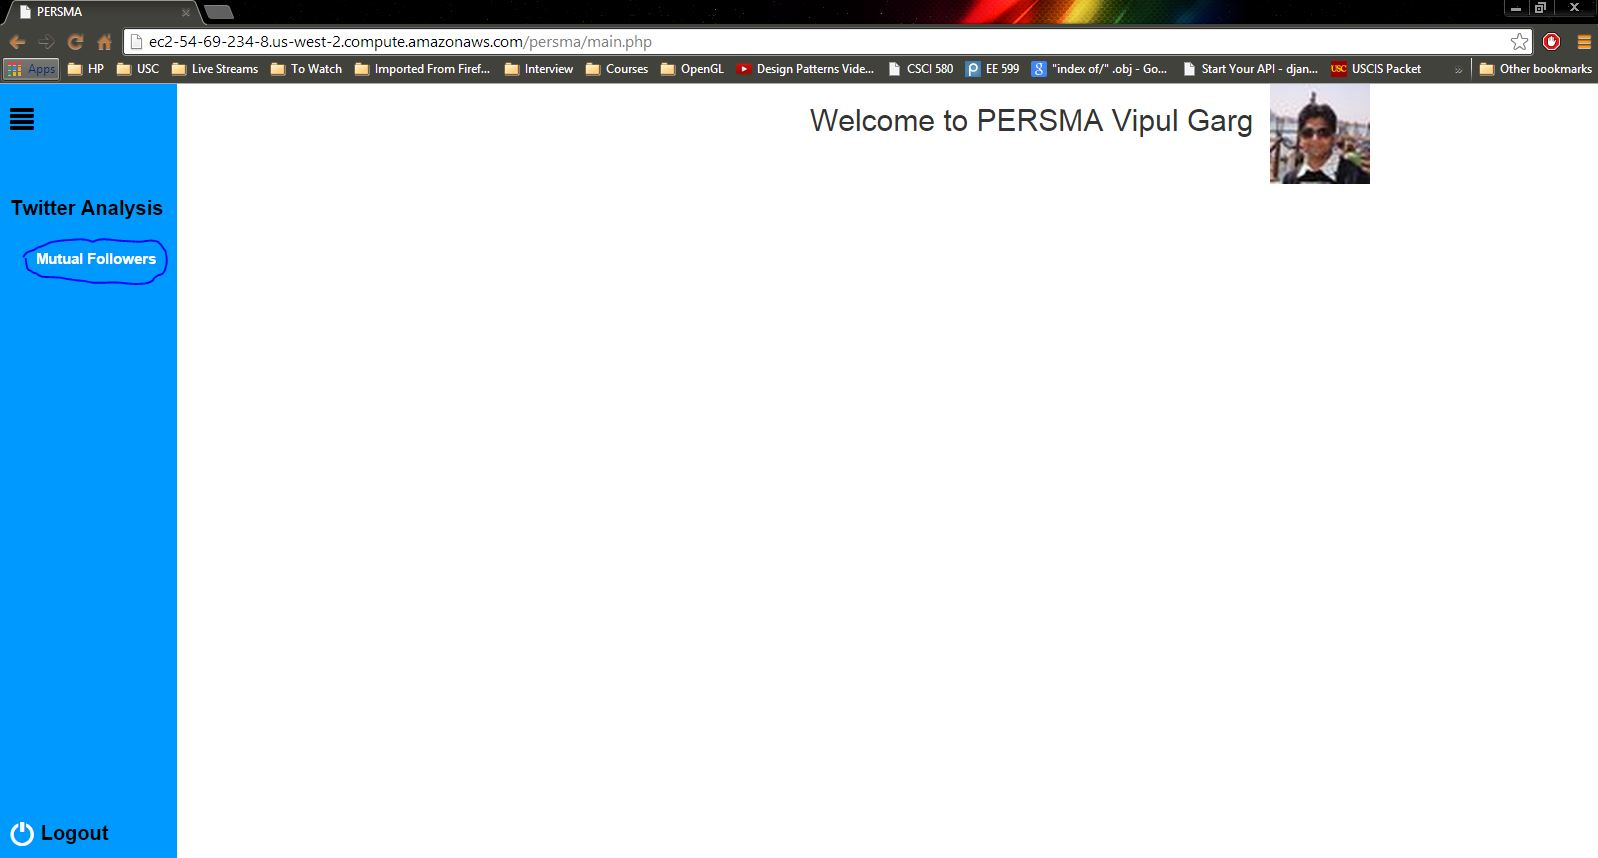
\includegraphics[height=40mm]{select_graph.JPG}
\captionfonts
\caption[Select a Graph]{Select a Graph}
\label{selectgraph}
\end{minipage}%
\end{figure}
Once the user selects the graph, the graph showing the mutual connectivity of the followers of the user is loaded onto the webpage as shown in figure \ref{graph1}. This graph is known as edge-bundling graph which is a type of circular layout. It depicts the first 14 followers of the user whose names are shown in a radially outward manner along the circumference of a circle. It also establishes relations between them by drawing a line between different followers to show links or edges between them. In Twitter, it is possible that a user follows another person but it is not necessary that the other person follows the same user back. This is depicted in the graph by the set of two blue lines, dark lines and bright lines. Dark lines represent that both the followers of the user follow each other and the bright lines represent that only one of them follows the other. This unidirectional relation becomes clearer by hovering the mouse over a particular person with a light edge. As can be seen in figure \ref{graph_highlighted}, there are two different kinds of lines visible from the graph, red lines and green lines. All the followers at the end of red lines are following the person on whom the mouse is currently hovering whereas the person on whom the mouse is hovering is following all users at the end of the green line emanating from her. This graph also has the ability to show communities within the graph. As can be seen, the user's graph has two distinct communities, where 5 followers of his(Paritosh, Rahil, Ashwini, Ravi and Nishant) are connected with each other and represent his Undergrad school community, and 3 other followers of his(Gulsheen, Shrikant and Jigar) are connected with each other representing his grad school community.\\
\begin{figure}[!htb]
\centering
\begin{minipage}[b]{0.45\linewidth}
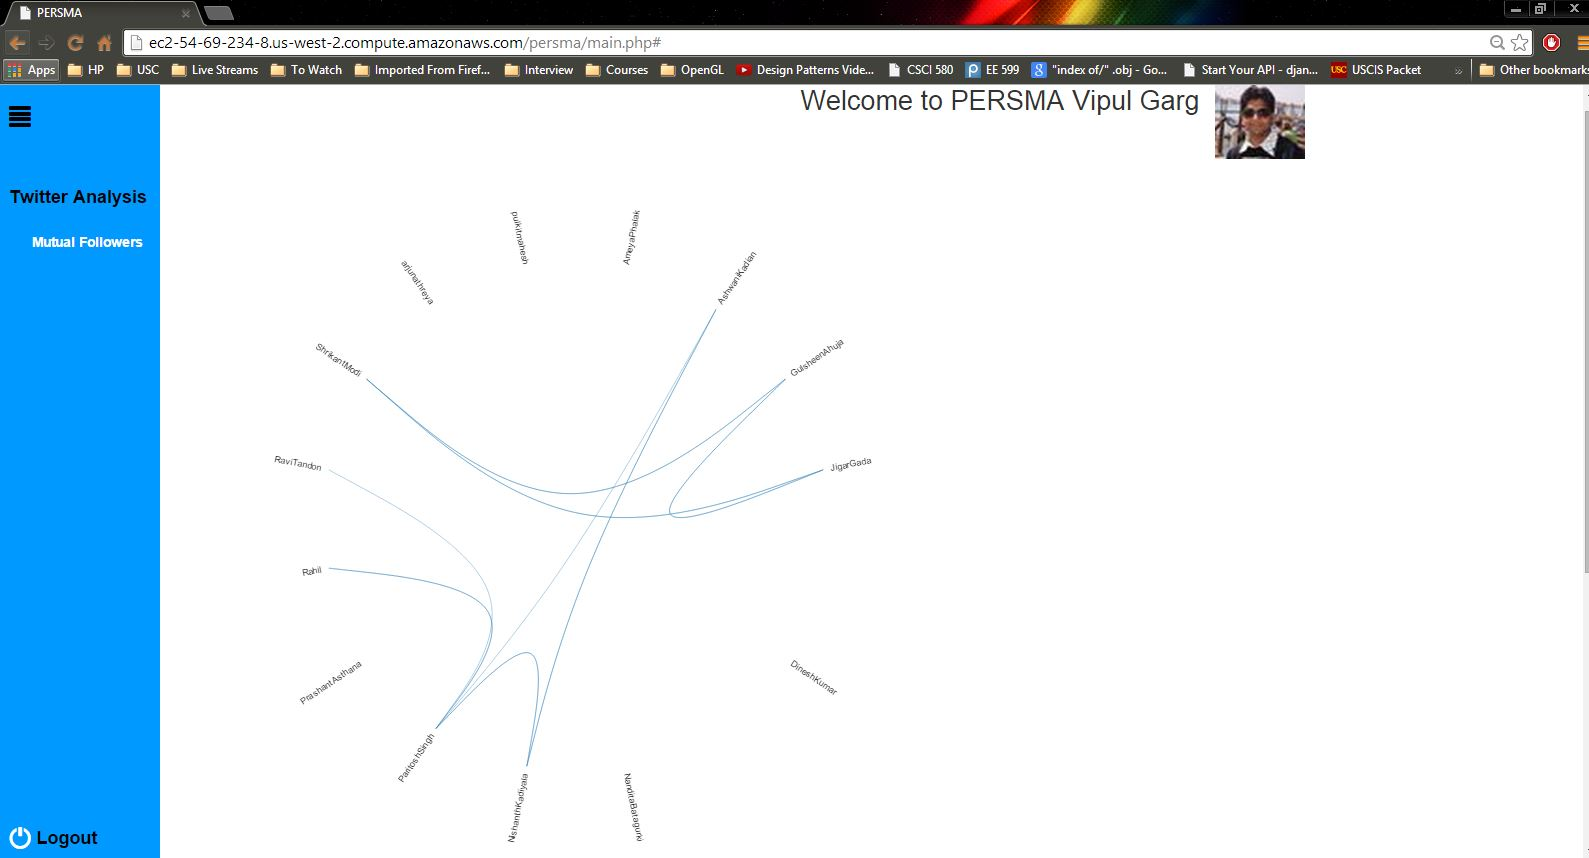
\includegraphics[height=40mm]{graph.JPG}
\captionfonts
\caption[Graph Displayed]{Graph Displayed}
\label{graph1}
\end{minipage}%
\begin{minipage}[b]{0.45\linewidth}
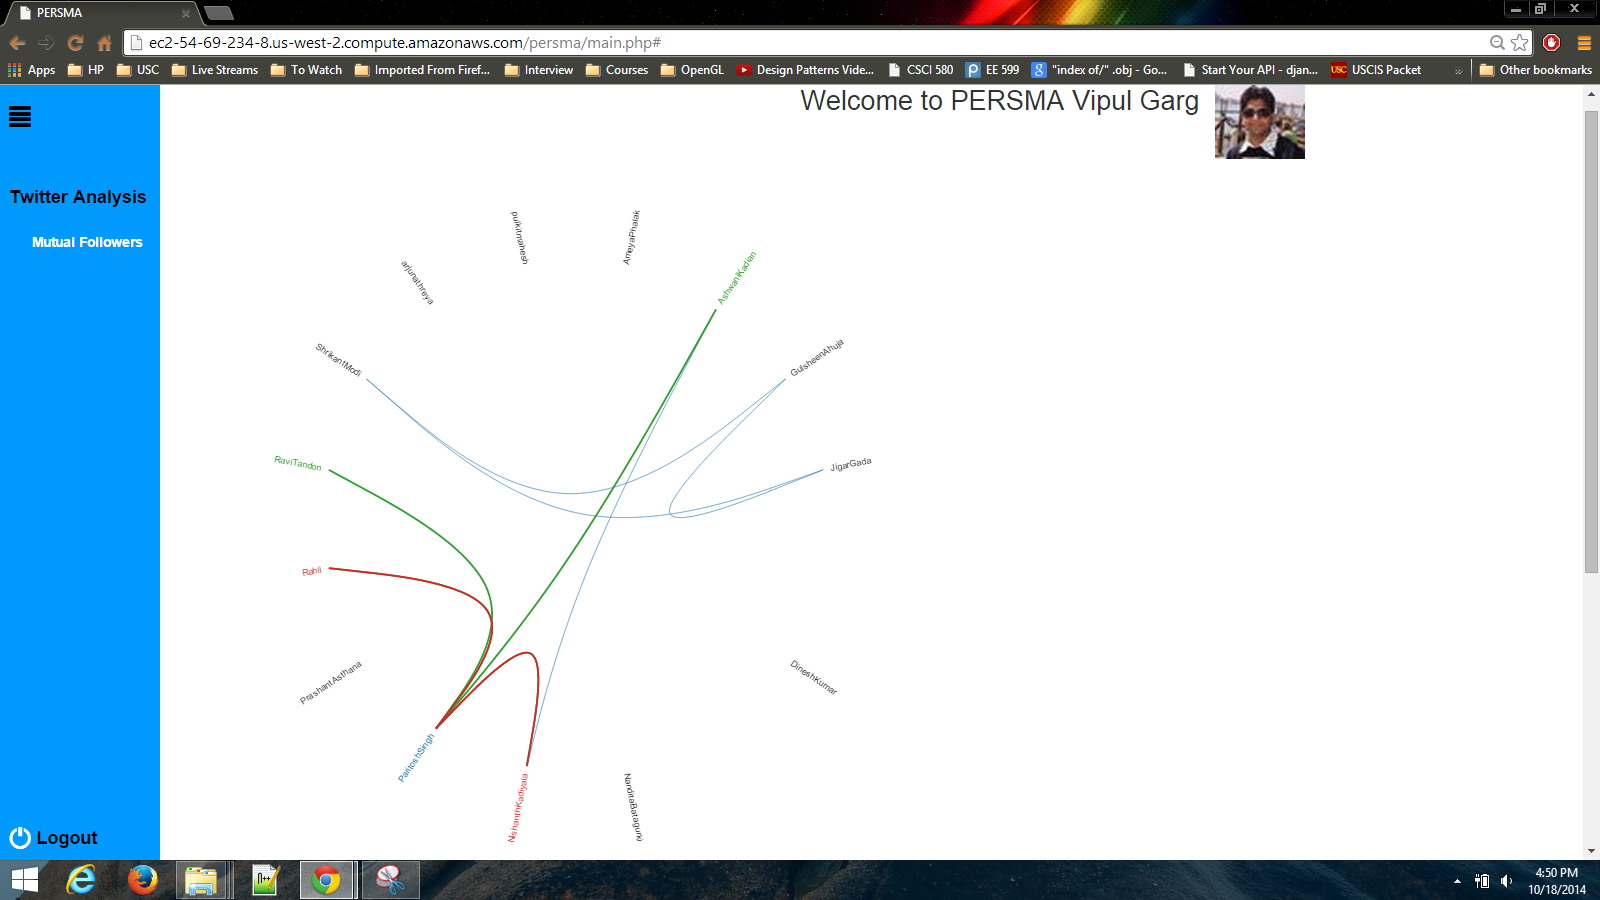
\includegraphics[height=40mm]{graph_highlighted.png}
\captionfonts
\caption[Highlighted Graph]{Highlighted Graph}
\label{graph_highlighted}
\end{minipage}
\end{figure}%

\chapter{Summary}
\label{Summary}
This project involved understanding different types of social media analysis tools available online for Facebook and Twitter. We found out that Wolfram's Facebook Personal Report provides a really detailed analysis about the user's network and her connections on Facebook, but it lacks a feature of predictive analysis which might be useful to the user. We also discussed similar tool for Twitter- Twitalyzer, which is used for analysis for the user's Twitter data. However, it is a paid service and it does not provide much predictive analysis of the user's data. Hence, we could figure out a need for a tool which can bridge the gap over existing tools.

As part of this project, we came up with a prototype for the tool which allowed the user to login via Twitter and then create a mutual relationship circular chart between the user's followers. 

The future work for the tool includes enhancing the tool's capabilities. We shall integrate the option of login via both Twitter and Facebook to extend the current charting capabilities. We shall also integrate the predictive analysis of the user's data from both Twitter and Facebook. All these features shall be done as part of Project 2.
% ------------- End main chapters ----------------------

\clearpage
\bibliography{bibliography}
\bibliographystyle{plain}
%\addcontentsline{toc}{chapter}{Bibliography}

\end{document}